%!TEX root=report.tex
\pagebreak
\subsection{LARS}

Below the full solution path of all the 39 coefficients is shown.
\begin{figure}[H]
\center
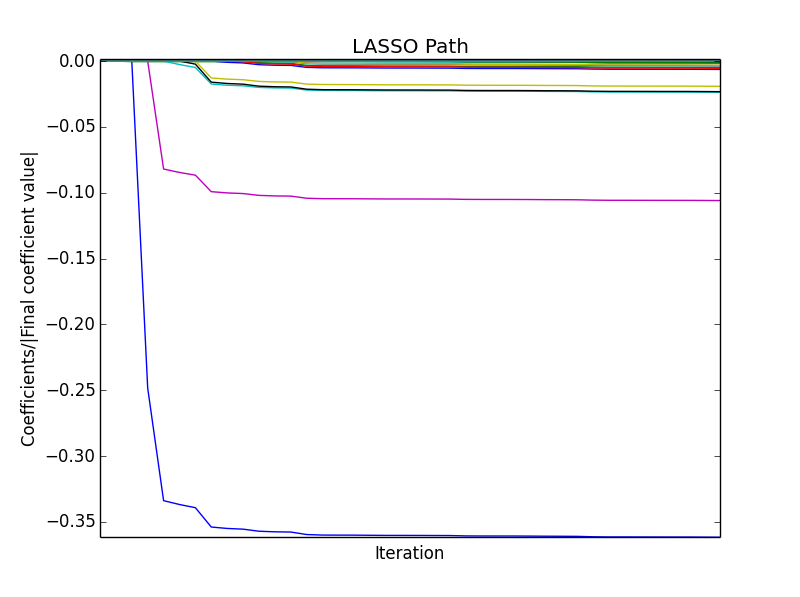
\includegraphics[width=10cm]{figures/lasso_path.png}
\caption{The above plot illustrates the coefficient path, for the solution corresponding to a point on the west coast of Greenland (coordinates [24,134]).}
\end{figure}
In the above plot it appears that after iteration 7 the coefficients doesn't really change that much. However since the lines are a bit to entangled to inspect visually, one can also plot the coefficent value divided by the final coefficient value, on the y axis:
\begin{figure}[H]
\center
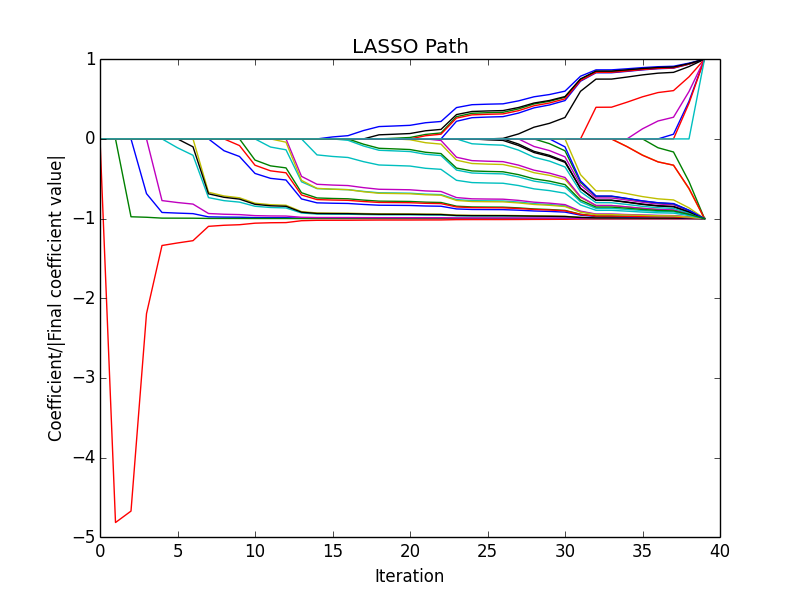
\includegraphics[width=8cm]{figures/lasso_path_scaled.png}
\caption{Scaled coefficients}
\end{figure}
\pagebreak
The 7 chosen coefficients and their values are :
\begin{lstlisting}[mathescape]

[ -3.53905876e-01  -4.28123366e-04  -1.13665156e-07  -1.74354380e-02  -9.91803076e-02  -1.28215596e-02  -1.60040198e-02]

[intercept (1), slope (t), acc. ($0.5  t^2$),$ cos(\frac{2\pi}{365.2 }t)$, $sin(\frac{2\pi}{365.2  }t)$, $cos( \frac{2\pi}{182.6  }t)$, $sin(\frac{2\pi}{182.6* t})$]
\end{lstlisting}
Using these 7 coefficients we get the following results:
\begin{figure}[H]
\center
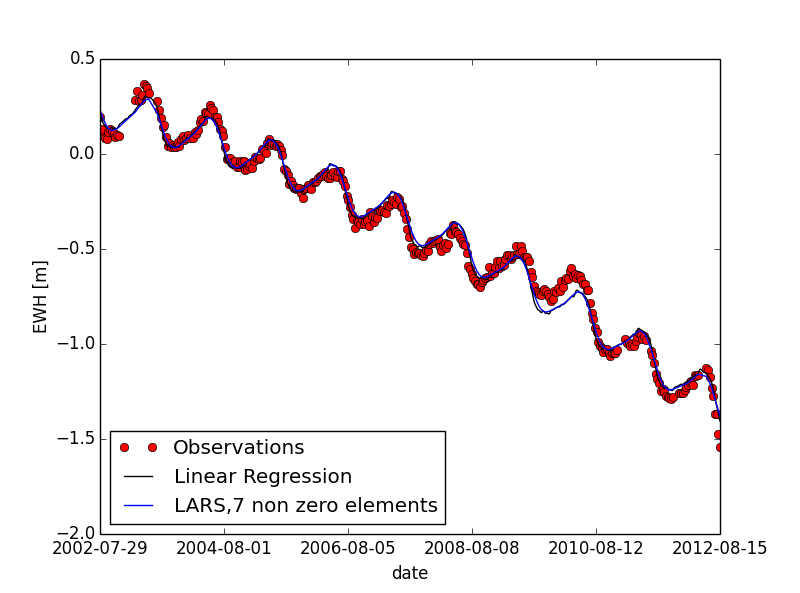
\includegraphics[width=10cm]{figures/lars_7.png}
\caption{It's evident from the graph that the LARS solution is very similar to the linear regression.}
\end{figure}

\subsubsection{How many frequencies are actually needed}

Ofcourse since this was only done for 1 point on the globe, if one were to apply this to other points one might get different lasso-paths and perhaps also a slight variance in the amount of coefficients needed. For example for modelling the ocean one wouldn't need as many coefficients, while potentially at places with heavy rain season, such as South America you might need more frequencies.
